\chapter{Isometric Force Characterization of Braided Pneumatic Actuators}\label{ch:muscles}\label{ch:methods}\label{ch:discussion}
\graphicspath{{../Figures/20-muscles/}}

{\doublespacing\normalsize\upshape
\noindent Publication note: Sections~\ref{sec:force_model}--\ref{sec:force_experiment}, Section~\ref{sec:results_force}, and Sections~\ref{sec:disc_effects}--\ref{sec:disc_bio}, with their associated figures and tables, appeared in \citet{bolen_2026} (Bolen, Elzein, Pang, and Hunt, \emph{Actuators}, 2026). For that work, B.B.\ performed the conceptualization, methodology, software, validation, formal analysis, investigation, data curation, visualization, and original draft preparation; M.E.\ and L.P.\ contributed methodology, software, investigation, and data curation; and A.H.\ supervised the work, administered the project, and acquired funding. All co-authors contributed to writing, review, and editing.\par}

This chapter develops and validates the actuator force models on which the rest of the dissertation builds, and it reads as one self-contained study, from methods through results to discussion. Sections~\ref{sec:force_model} and~\ref{sec:force_experiment} present the methods: the force equations used throughout this work, and the test jig and measurement procedure used to characterize Festo BPAs with \qtylist{10;20}{\mm} uninflated diameters over a wide range of resting lengths, contractions, and pressures. Section~\ref{sec:results_force} reports the resulting maximum-force and normalized force--strain--pressure models and compares them with the manufacturer's tool. The remaining sections discuss the effects of resting length, the nondimensionalized force prediction, the comparison with other published BPA models, the implications for real-time control and simulation, and the analogy between these artificial muscles and biological muscle. The validated force model is the one used for the knee-torque predictions of Chapter~\ref{ch:torque} and for the BPA actuation of the neuromechanical simulations in Chapter~\ref{ch:sns}.

\section{Methods}

\subsection{Actuator Force Model}\label{sec:force_model}


The actuator force model used throughout this dissertation is described here. First, the amount of contraction ${\varepsilon}$ in a BPA is calculated as

\begin{equation}
    {\varepsilon} = \frac{(l_{0}-l_\text{m})}{l_{0}} \label{eq:strain}
\end{equation}

where $l_{0}$ is uninflated resting length of the BPA measured from hose clamp to hose clamp. Current muscle length is $l_\text{m}$.

Similarly, ${\varepsilon_{620}}$ is the amount of contraction in a BPA without external load when inflated at $\qty{620}{\kPa}$, calculated as 

\begin{equation}
    \varepsilon_{620} = \frac{(l_{0}-l_{620})}{l_{0}} \label{eq:max_strain}
\end{equation}

where $l_{620}$ is the muscle length measured at \qty{620}{\kPa} and free from external loads. 

The amount of relative contraction of a BPA $\varepsilon^*$ can then be calculated by dividing equation \eqref{eq:strain} by \eqref{eq:max_strain}, such that

\begin{equation}
    \varepsilon^* = \frac{\varepsilon}{\varepsilon_{620}} \label{eq:rel_strain}
\end{equation}

describes the BPA's current contraction as a normalized percentage of its total.

The amount of normalized isometric force $F^*$ in a Festo BPA is then calculated as
\begin{equation}
F^*(\varepsilon^*,P^*)=
\begin{cases}
\begin{aligned}
c_0\cdot\bigl(\exp(-c_1 \cdot \varepsilon^*)-1\bigr)
+ P^*\cdot\exp\!\bigl(-c_2(\varepsilon^*)^{2}\bigr)
\end{aligned}
& \text{for } F^*>0\\[10pt]
0
& \text{for } F^*\le 0
\end{cases}\label{eq:Fstar}
\end{equation}

where $P^*$ is pressure $P$ normalized by \qty{620}{\kPa}. BPA diameter dependent coefficients are determined by the actuator characterization experiments reported in Section~\ref{sec:results_force} (Table~\ref{tab:Fstar}).

The maximum force $F_{max}$ in a BPA is calculated as

\begin{equation}
    F_{max}(l_{0},P_\text{max}) = a_1 \cdot P \cdot \arctan{(a_2 \cdot P \cdot (l_{0}-0.0075))} \label{eq:Fmax_3D}
\end{equation}

with coefficients determined by the actuator characterization experiments reported in Section~\ref{sec:results_force} (Table~\ref{tab:Fmax}). When maximum system pressure is set to $P=\qty{620}{\kPa}$, $F_\text{max}(l_{0},620) = F_{620}(l_{0})$. Multiplying \eqref{eq:Fstar} by \eqref{eq:Fmax_3D} yields

 \begin{equation}
   F(\varepsilon^*,P^*,l_{0}) = F^*(\varepsilon^*,P^*) \cdot F_{620}(l_{0}) \label{eq:force}
\end{equation}

as the equation for isometric force $F$ in a Festo BPA.

\subsection{BPA Isometric Force Characterization Experiment}\label{sec:force_experiment}


To measure artificial muscle force as a function of length and pressure, we built a test jig from extruded aluminum and 3D printed parts. Festo BPAs with \qtylist{10;20}{\mm} diameter were tested with various resting lengths and different amounts of contraction. These data are used to develop an improved model that more accurately predicts maximum muscle force based on $l_0$, current muscle length $l_{m}$, and pressure $P$. The results are compared with existing models and the new data are used to create an updated model. 

A test jig was made of 80/20 brand 1515 series extruded aluminum (Figure~\ref{fig:testJig}). Artificial muscles were placed vertically in the jig one at a time. The upper end was attached to a load cell.
Force data was collected using a CALT DYLY-103 100 kg S-shaped load cell for the $\diameter$\qty{10}{\mm} BPAs and a Loadstar RAS1-2HKS-S for the $\diameter$\qty{20}{\mm} BPAs. The load cell was used in conjunction with a HX711 Load Cell Amplifier. Pressure data was obtained from a Freescale MPX5700 GP \qty{5}{\volt} pressure sensor. Building air supply pressure was controlled with two pressure regulators in series. The first was a Parker model 20R113GC $0-120\,\text{psi}$ pressure regulator. The second was a Husky $3/8\,\text{in.}$ High Performance Air Regulator HDA72200. A Festo VTUG-10-MRCR-S1T-26V20-T516LA-UL-532S-8K valve manifold VTUG-G was used to deliver air from the pressure regulator to the actuator. This manifold is comprised of eight two-in-one bidirectional normally closed Festo VUVG-S10-T32C-AZT-M5-1T1L valves. 

Pressure and load cell amplifier data were sent to MATLAB 2021b via an Arduino Uno style Sparkfun BlackBoard C microcontroller. The computers that used MATLAB were running either Windows 10 or Windows 11. During phases when the Arduino was collecting force and pressure data to send to MATLAB, the Arduino would also trigger (via MATLAB) an Onsemi 2N4401 NPN transistor to make the valve manifold open or close the valve. For other data collection, the valve was manually opened and closed. 

The inner distance between the hose clamps on each BPA was measured with a FANUC tape measure to determine the muscle's length $l$ and resting length ($l_0$). This is how \citet{festo_2026} defines $l_0$, although in \citet{hunt_modeling_2017} it was measured to also include end cap length. We then inflated each BPA to $P_{620}=\qty{620}{kPa}$, with one end allowed to move freely in the axial Degree of Freedom (DoF), and measured the length $l_{620}$ to calculate maximum contraction at \qty{620}{\kPa} using Equation~(\ref{eq:max_strain}). The distance between the crossmembers was then controlled to obtain different amounts of contraction, the muscles were inflated to various pressures, and the contractile force was recorded at the pressure--contraction pairs. This was done for $\diameter$\qty{10}{\mm} BPA resting lengths ($l_0$) of \SIrange[range-phrase=--]{112}{518}{\mm}. For $\diameter$\qty{20}{\mm} BPAs, resting lengths ($l_0$) of \SIrange[range-phrase=--]{300}{509}{\mm} were used.

\begin{figure}[htbp]
   \begin{center}
   \hspace{-11mm} 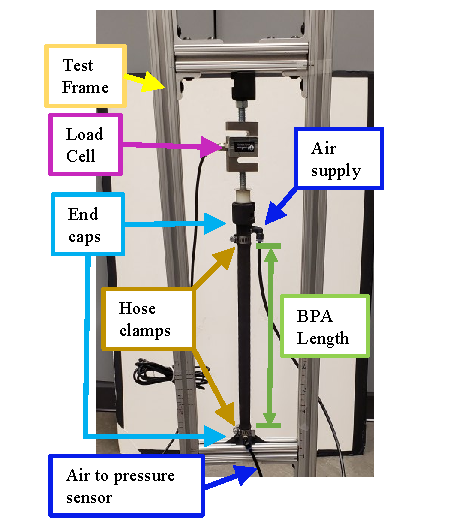
\includegraphics[width=0.75\textwidth]{01_testJigs1.pdf}
   \end{center}
    \caption{A picture of a BPA in the isometric force test stand with components labeled.}\label{fig:testJig}
\end{figure}

\section{Results}

\subsection{BPA Force Characterization}\label{sec:results_force}

This section reports the results of the isometric force characterization experiments described in Section~\ref{sec:force_experiment}. First, maximum isometric force at \qty{620}{\kPa} is modeled as a function of resting length. The remaining data are then normalized to build a predictive force surface, and the resulting model is compared with the manufacturer's tool and with other published BPA models.


\subsubsection{Maximum Force at 620 kPa}

Data of the maximum force from BPA characterization tests of the \qty{10}{\mm} and \qty{20}{\mm} diameters at \qty{620}{\kPa} show a dependency on resting length (Figure~\ref{fig:Fmax_fit}). This is a previously unreported characteristic of these artificial muscles. Detailed analysis of the Festo \mbox{tool \citep{festo_2026}} does in fact predict a change in maximum force with the resting length; however, the Festo tool predicts increased force with shorter lengths, while our collected data indicate decreasing force with shorter lengths. The data show a force response resembling an $\arctan$ curve along the $l_0$ dimension. Using the Nonlinear Least Squares method and a Least Absolute Residual robustness, we fit an arctan curve to the data to get the maximum force at \qty{620}{\kPa} given a resting length as:
\begin{align}
    F_{620_{10}} &= \qty{303.5}{\N}\cdot \arctan{( \qty{19.03}{\per\metre} \cdot (l_0-0.0075))}  \label{eq:Fmax10} \\[10pt]
    F_{620_{20}} &= \qty{922.4}{\N} \cdot \arctan{(\qty{15.37}{\per\m} \cdot (l_0-0.013))} \label{eq:Fmax20}
\end{align}

\noindent
The length is offset by \qty{0.0075}{\m} and \qty{0.013}{\m} because solid modeling showed that the end caps contact each other at these lengths. At these lengths, the actuator would not be able to contract to produce force.


\begin{figure}[H]%[tbp]
%\begin{adjustwidth}{-\extralength}{0cm}
%\centering
\subfloat[\centering]{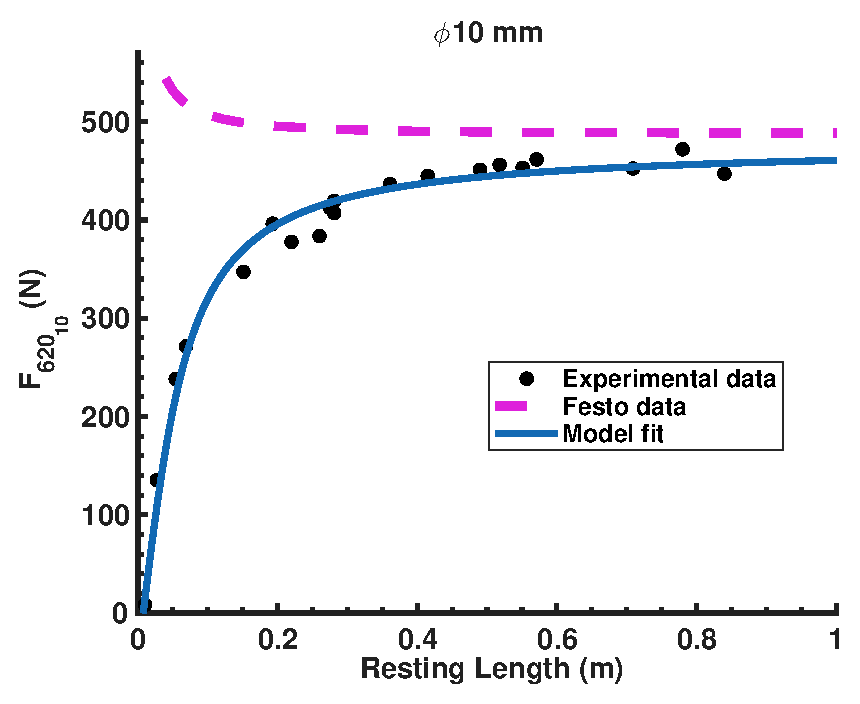
\includegraphics[width=13.8cm]{02a_MaxForce10.eps}}\\
\subfloat[\centering]{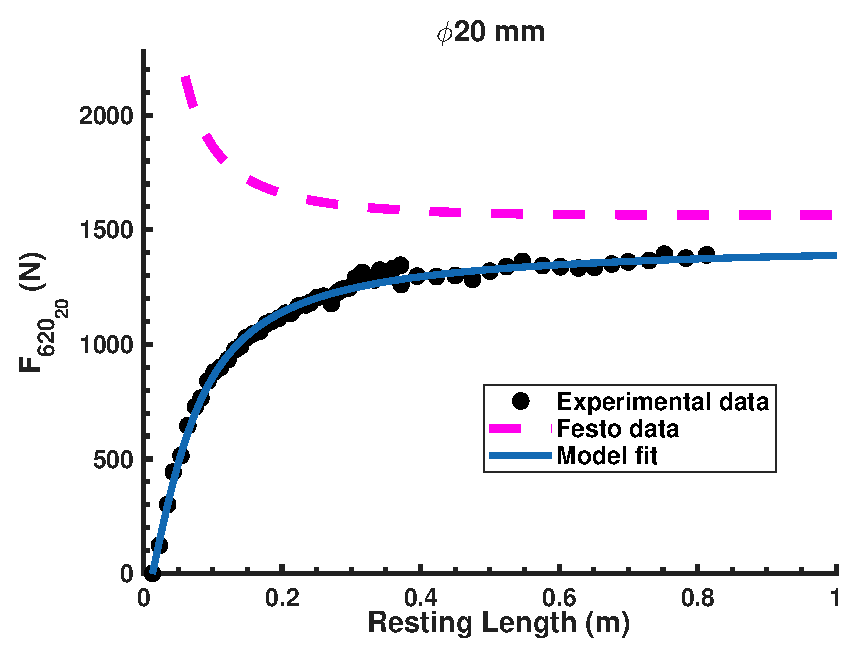
\includegraphics[width=13.8cm]{02b_MaxForce20.eps}}
%\includegraphics[width=1\textwidth]{02_Fmax_fit.eps}
%\end{adjustwidth}
\caption{Results for finding the relationship between $F_{620}$ and $l_0$. (\textbf{a}) $F_{620_{10}}$ as a function of $l_0$, at $P_{620}$. Dashed line is the $F_{620_{10}}$ data from Festo. Solid line is the fit from Equation (\ref{eq:Fmax10}). (\textbf{b}) $F_{620_{20}}$ as a function of $l_0$ at $P_{620}$. Dashed line is $F_{620_{20}}$ data from Festo. Solid line is the fit from Equation (\ref{eq:Fmax20}).}\label{fig:Fmax_fit}
\end{figure}

\subsubsection{Force as a Function of Pressure and Resting Length}

Data from BPA characterization tests of the \qty{10}{\mm} muscles resulted in force--pressure pairings for different muscle resting lengths ($l_0$) (Figure~\ref{fig:F-P_contraction}a). Similar to the maximum force data, these data show a force response resembling an $\arctan$ curve along the $l_0$ dimension  with a more linear response to changes in pressure. Using the Nonlinear Least Squares method and a Least Absolute Residual robustness, we fit an arctan curve to the data to get the maximum force given a resting length and pressure as described by the model form given in Section~\ref{sec:force_model},
where $a_1 = \qty{0.4895}{\N\per\kPa}$  and $a_2=\qty{0.03068}{\per\kPa\per\m}$ for the \qty{10}{\mm} actuator, and \mbox{$a_1 = \qty{1.49}{\N\per\kPa}$,} $a_2=\qty{0.0248}{\per\kPa\per\m}$ for the \qty{20}{\mm} actuator. Goodness-of-fit measures are given in Table~\ref{tab:Fmax}; throughout this dissertation, goodness of fit is reported as the root-mean-square error (RMSE), the adjusted fraction of variance unexplained (FVU, for which $R^{2} = 1 - \mathrm{FVU}$), and the maximum absolute residual, as defined alongside the reference implementation in Appendix~\ref{app:muscle_calcs}. 



\begin{sidewaystable}[p]
\centering
\begingroup
\singlespacing
\fontsize{10}{12}\selectfont
\setlength{\tabcolsep}{3pt}
\renewcommand{\arraystretch}{1.15}
\caption{Maximum force equation coefficient values with confidence intervals (CI) and goodness-of-fit measures. Equation~(\ref{eq:Fmax_3D}) is compared to data taken at \qty{620}{\kPa}. Equations~(\ref{eq:Fmax10}) and (\ref{eq:Fmax20}) are compared against maximum force from using the Festo tool. It was not necessary to fit an adjusted $\text{R}^2$ in \mbox{these cases.}} 
\label{tab:Fmax}
\begin{tabular}{@{}cllrrrrrr@{}}
\toprule
\multirow{2}{*}{\textbf{Equation}} &
  \multirow{2}{*}{\textbf{Coefficient}} &
  \multirow{2}{*}{\textbf{CI (95\%)}} &
  \multicolumn{3}{c}{\textbf{Our Model}} &
  \multicolumn{3}{c}{\textbf{Festo Tool}} \\  
 &
   &
   &
  \multicolumn{1}{l}{\textbf{Adj. $\text{R}^2$}} &
  \multicolumn{1}{l}{\textbf{RMSE}} &
  \textbf{Max. Error} &
  \multicolumn{1}{l}{\textbf{Adj. $\text{R}^2$}} &
  \multicolumn{1}{l}{\textbf{RMSE}} &
  \textbf{Max. Error} \\ \midrule 
\multirow{2}{*}{\eqref{eq:Fmax_3D}} &
  $a_1 =   \qty{0.4895}{\N\per\kPa}$ &
  (0.4822, 0.4968) &
  \multicolumn{1}{l}{\multirow{2}{*}{0.9945}} &
  \multicolumn{1}{l}{\multirow{2}{*}{11.61 N}} &
  \multirow{2}{*}{55.3 N} &
  \multicolumn{1}{l}{\multirow{2}{*}{0.9854}} &
  \multicolumn{1}{l}{\multirow{2}{*}{14.7 N}} &
  \multirow{2}{*}{30.9 N} \\ 
 &
  $a_2 =   \qty{0.03068}{\per\kPa\per\m}$ &
  (0.0282, 0.03317) &
  \multicolumn{1}{l}{} &
  \multicolumn{1}{l}{} &
   &
  \multicolumn{1}{l}{} &
  \multicolumn{1}{l}{} &
   \\ \midrule
\multirow{2}{*}{\eqref{eq:Fmax10}} &
  $b_1   =\qty{303.5}{\N}$ &
  (300, 308) &
  \multicolumn{1}{l}{\multirow{2}{*}{0.9854}} &
  \multicolumn{1}{l}{\multirow{2}{*}{14.72 N}} &
  \multirow{2}{*}{30.9 N} &
  \multicolumn{1}{c}{\multirow{2}{*}{--}} &
  \multicolumn{1}{l}{\multirow{2}{*}{189.9 N}} &
  \multirow{2}{*}{375.6 N} \\ 
 &
  $b_2 =   \qty{19.03}{\per\m}$ &
  (17.48, 20.57) &
  \multicolumn{1}{l}{} &
  \multicolumn{1}{l}{} &
   &
  \multicolumn{1}{l}{} &
  \multicolumn{1}{l}{} &
   \\ \midrule
\multirow{2}{*}{\eqref{eq:Fmax20}} &
  $b_1 =   \qty{922.4}{\N}$ &
  (914.2, 930.7) &
  \multicolumn{1}{l}{\multirow{2}{*}{0.9945}} &
  \multicolumn{1}{l}{\multirow{2}{*}{23.83 N}} &
  \multirow{2}{*}{62.1 N} &
  \multicolumn{1}{c}{\multirow{2}{*}{--}} &
  \multicolumn{1}{l}{\multirow{2}{*}{668.4 N}} &
  \multirow{2}{*}{1590.1 N} \\ 
 &
  $b_2=\qty{15.37}{\per\m}$ &
  (14.75, 15.98) &
  \multicolumn{1}{l}{} &
  \multicolumn{1}{l}{} &
   &
  \multicolumn{1}{l}{} &
  \multicolumn{1}{l}{} &
   \\ \bottomrule
\end{tabular}

\vspace{1.5em}
\caption{Normalized isometric BPA force equation (Equation~(\ref{eq:Fstar})) coefficient values and goodness-of-fit measures.}
\label{tab:Fstar}
\begin{tabular}{@{}cllrrrrrr@{}}
\toprule
\multirow{2}{*}{\textbf{BPA}} &
  \multirow{2}{*}{\textbf{Coefficient}} &
  \multirow{2}{*}{\textbf{CI (95\%)}} &
  \multicolumn{3}{c}{\textbf{Model}} &
  \multicolumn{3}{c}{\textbf{Validation}} \\ 
& & &
  \multicolumn{1}{l}{\textbf{Adj. $\text{R}^2$}} &
  \multicolumn{1}{l}{\textbf{RMSE}} &
  \textbf{Max. Error} &
  \multicolumn{1}{l}{\textbf{Adj. $\text{R}^2$}} &
  \multicolumn{1}{l}{\textbf{RMSE}} &
  \textbf{Max. Error} \\ \midrule
\multirow{3}{*}{$\diameter$\qty{10}{\mm}} &
  $c_0 = 0.5682$ & (0.5584, 0.578) &
  \multicolumn{1}{l}{\multirow{3}{*}{0.9998}} &
  \multicolumn{1}{l}{\multirow{3}{*}{0.005118}} &
  \multirow{3}{*}{10.3\%} &
  \multicolumn{1}{l}{\multirow{3}{*}{0.9994}} &
  \multicolumn{1}{l}{\multirow{3}{*}{0.0245409}} &
  \multirow{3}{*}{10.6\%} \\ \cmidrule{2-3}
& $c_1 = 4.254$ & (4.126, 4.383) &
  \multicolumn{1}{l}{} & \multicolumn{1}{l}{} & &
  \multicolumn{1}{l}{} & \multicolumn{1}{l}{} & \\ \cmidrule{2-3}
& $c_2 = 0.5597$ & (0.5429, 0.5766) &
  \multicolumn{1}{l}{} & \multicolumn{1}{l}{} & &
  \multicolumn{1}{l}{} & \multicolumn{1}{l}{} & \\ \midrule
\multirow{3}{*}{$\diameter$\qty{20}{\mm}} &
  $c_0 = 0.2579$ & (0.2401, 0.2756) &
  \multicolumn{1}{l}{\multirow{3}{*}{0.992}} &
  \multicolumn{1}{l}{\multirow{3}{*}{0.02294}} &
  \multirow{3}{*}{6.8\%} &
  \multicolumn{1}{l}{\multirow{3}{*}{0.9943}} &
  \multicolumn{1}{l}{\multirow{3}{*}{0.0231303}} &
  \multirow{3}{*}{5.7\%} \\ \cmidrule{2-3}
& $c_1 = 6.477$ & (5.558, 7.396) &
  \multicolumn{1}{l}{} & \multicolumn{1}{l}{} & &
  \multicolumn{1}{l}{} & \multicolumn{1}{l}{} & \\ \cmidrule{2-3}
& $c_2 = 1.321$ & (1.239, 1.403) &
\multicolumn{1}{l}{} & \multicolumn{1}{l}{} & &
\multicolumn{1}{l}{} & \multicolumn{1}{l}{} & \\ \bottomrule
\end{tabular}

\endgroup
\end{sidewaystable}



\subsubsection{Maximum Contraction at \qty{620}{\kPa}}

Figure~\ref{fig:F-P_contraction}(b) shows an attempt at a linear fit for maximum contraction at \qty{620}{\kPa} ($\epsilon_{620}$) as a function of resting length ($l_0$). Error bars have been included to show the effect of $\pm$\qty{1}{\mm} accuracy with measurements of $l_0$ and $l_{620}$. There was a large amount of variance in the data, with the linear fit giving an adjusted $\text{R}^2=0.4124$ and an $\text{RMSE}=0.0083$. Since there is no direct, predicable relationship between maximum contraction and $l_0$, this value should be recorded in each muscle used on a robot to best predict the force it may produce at different pressures and contraction. 


\subsubsection{Force as a Function of Pressure and Contraction}

In addition to being a function of the pressure and resting length, the force produced by the actuator is also a function of the amount of actuator contraction, with less force being applied as the actuator contracts. 
To build this model, the collected data of force, pressure, and contraction are normalized by dividing by $F_{620}$, $P_{620}$, and $\epsilon_{620}$, respectively. This had the effect of compressing the data into a 3D surface ranging from 0 to 1 on all axes. Normalized data are compared with pressure isoclines of force predicted by the Festo tool divided by the maximum force equation described in the previous section in Figure~\ref{fig:GenForceFit}. With this comparison, it is clear that the Festo tool over-predicts the expected force, especially at lower pressures, contraction, and resting lengths.  






\begin{figure}[H]%[tbp]
%\begin{adjustwidth}{-\extralength}{0cm}
%\centering
\subfloat[\centering]{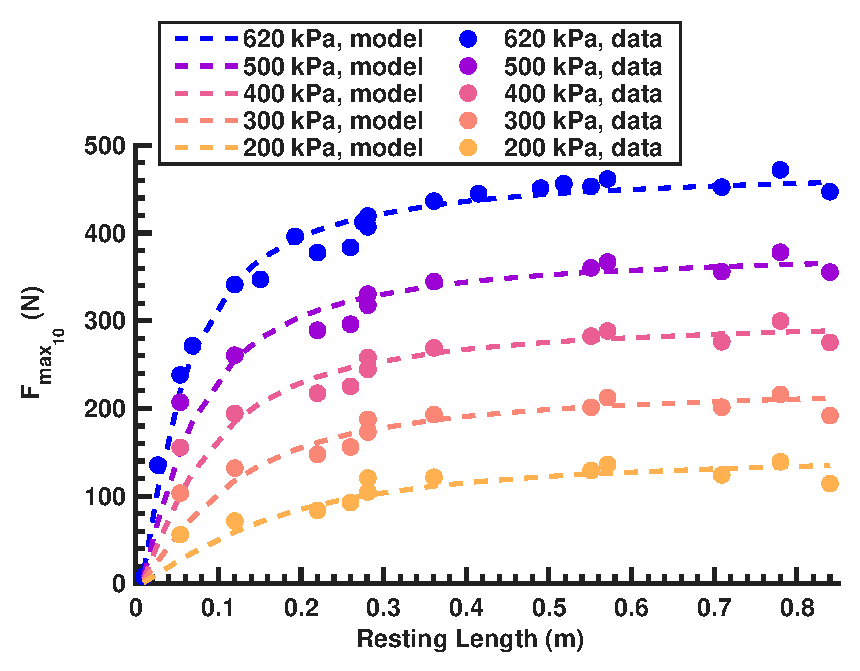
\includegraphics[width=13.3cm]{03a_MaxForce10_all.eps}}\\
\subfloat[\centering]{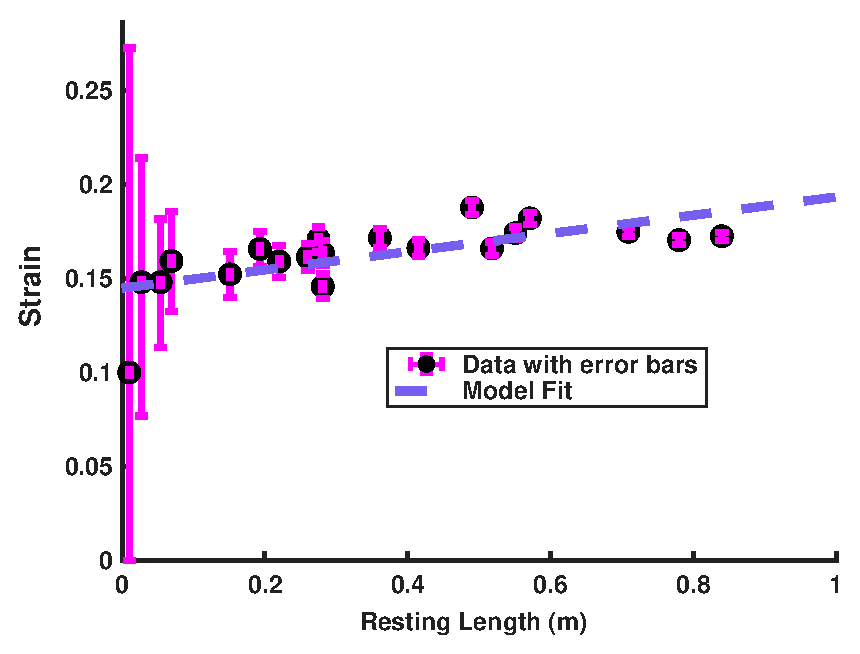
\includegraphics[width=13.8cm]{03b_kmax10.eps}}
%\end{adjustwidth}
\caption{Results for finding the relationship between $F_{620}$, $l_0$, $P_{620}$, and $\epsilon_{620_{10}}$. (\textbf{a}) Isoclines of the surface fit for $F_{620_{10}}(l_0,P_{620})$. (\textbf{b}) $\epsilon_{620_{10}}$ versus $l_0$ at $P_{620}$. Although there is a general trend of longer resting lengths producing more contraction, no conclusive relationship between $\epsilon_{620}$ and $l_0$ could be deduced from this experiment. The error bars show the effect of being $\pm$\qty{1}{\mm} in measuring $l_0$ and $l_{620}$.}\label{fig:F-P_contraction}
\end{figure}





\begin{figure}[H]%[tbp]
%\begin{adjustwidth}{-\extralength}{0cm}
%\centering
\subfloat[\centering]{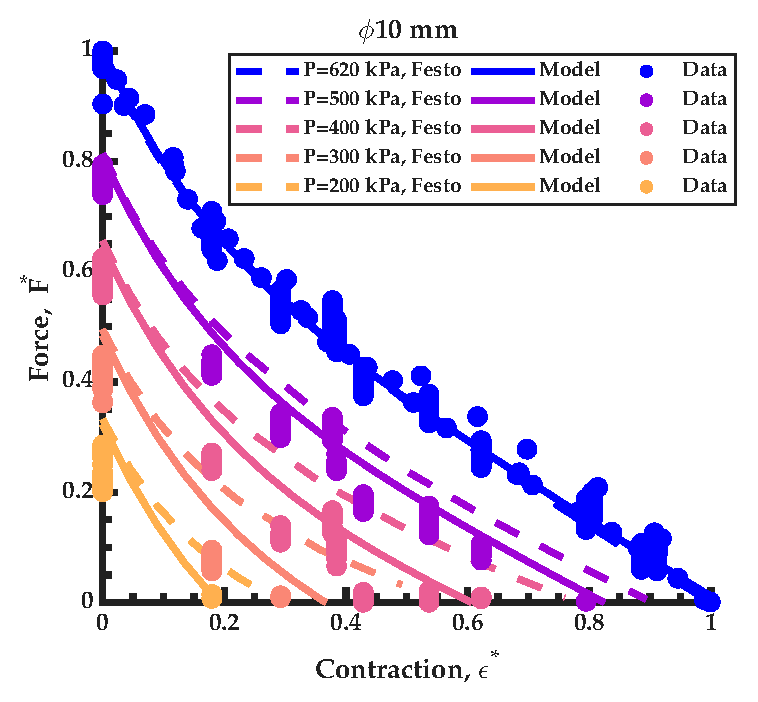
\includegraphics[width=10.88cm]{04a_FStar10.eps}}\\
\subfloat[\centering]{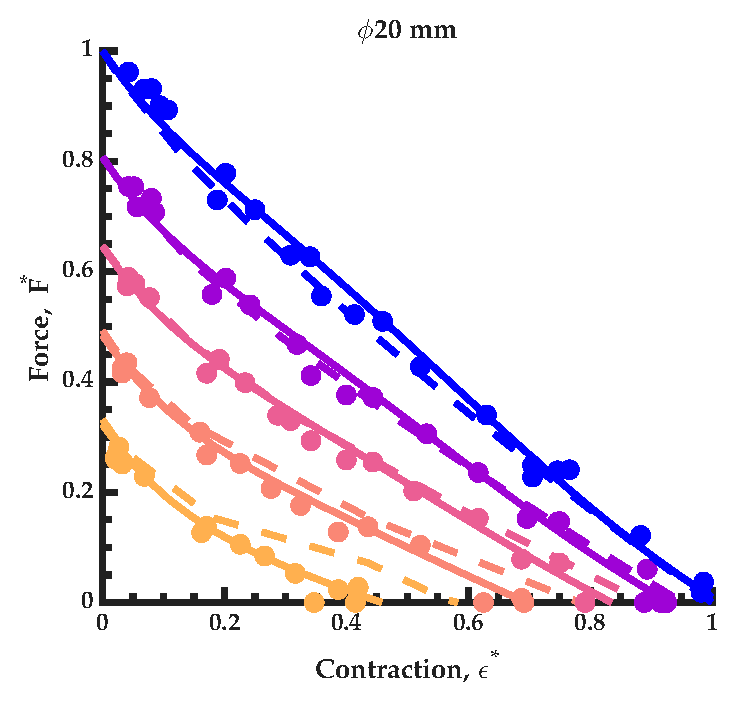
\includegraphics[width=10.88cm]{04b_FStar20.eps}}
%\end{adjustwidth}
\caption{Surface fit for $F^*(\epsilon^*,P^*)$. Solid lines are from our model. Dashed lines from Festo supplied data. In total, 537 data points were collected and used to fit the 3D surfaces (321 data points for $\diameter$\qty{10}{\mm} BPAs and 216 data points for $\diameter$\qty{20}{\mm} BPAs). In total, 80\% of these data were used for training, and 20\% were used for validation. For figure clarity, not all data is included and plotted circles represent collected data at $\pm\qty{10}{\kPa}$ of the stated pressure. (\textbf{a}) Fit data for $\diameter$\qty{10}{\mm} Festo BPAs. (\textbf{b}) Fit data for $\diameter$\qty{20}{\mm} Festo BPAs.}\label{fig:GenForceFit}
\end{figure}

We therefore derived our own equation for isometric force in the BPA as a function of pressure and contraction. Visual analysis of the experimental data shows an exponential relationship between $\epsilon^*$ and $F^*$, and a linear relationship between $P^*$ and $F$. We fit a surface to the data using Nonlinear Least Squares and a Least Absolute Residual robustness such that it is described by 
Equation~\eqref{eq:Fstar}.
For the $\diameter$\qty{10}{\mm} BPAs, the result of the improved fit can be seen in Figure \ref{fig:GenForceFit}a. The adjusted $\text{R}^2=0.9998$, a $\text{RMSE}=0.004537$, and a maximum absolute residual of $10.6\%$. Solving (\ref{eq:Fstar}) for the $\diameter$\qty{20}{\mm} BPA, yields different coefficients, and results are seen in \mbox{Figure~\ref{fig:GenForceFit}b.} Coefficient values and goodness-of-fit statistics are found in Table \ref{tab:Fstar}. 











\section{Discussion}

\subsection{Effects of Resting Length}\label{sec:disc_effects}
We have developed new $F_{620}$ equations for \qtylist{10;20}{\mm} diameter Festo BPAs that capture the change in maximum force produced by the actuators at  \qty{620}{\kPa} as a function of their resting length. When examining Equation~(\ref{eq:Fmax10}) and measured data in Figure~\ref{fig:Fmax_fit}b, it can be seen that as $l_0$ goes to infinity, $F_{620_{10}}$ goes to \qty{470}{\N}. When the Festo tool \citep{lang_robert_musclesim_2005} was queried at $l_0=\qty{1}{m}$ as an approximation of infinity, it predicts the $\diameter$\qty{10}{\mm} BPA can produce $F=\qty{490}{\N}$ at $P_{620}$. This is within the 10\% variability that Festo states may occur in manufacturing tolerances. Similarly, the Festo data predict a $\diameter$\qty{20}{\mm} BPA will produce $F=\qty{1570}{\N}$. Our results for Equation~(\ref{eq:Fmax20}) show that  $F_{620_{20}}$ goes to \qty{1460}{\N} as $l_0$ approaches infinity. Although the difference is much larger, it is also within the \mbox{10\% manufacturing tolerance. }

Our measured data differ significantly from the Festo model as $l_0$ goes to zero. For the measured data, as the length gets smaller, the force does as well, whereas the Festo tool predicts exponential force increase (see Figure~\ref{fig:Fmax_fit}). As a specific example, when specifying $l_0=\qty{112}{\mm}$ for the \qtylist{10}{\mm} diameter BPAs, the Festo predicted $F_{620}$ is \qtylist{498.6}{\N}. However, using Equation~(\ref{eq:Fmax10}), $F_{620}$ is calculated to be \qtylist{335.3}{\N}. Actual force in the $l_0=\qty{112}{\mm}$ was measured at \qtylist{350.9}{\N}. Therefore, the error in predicted $F_{620}$ for the $\diameter$\qty{10}{\mm} BPA is $4.5\%$ for our model and $42.1\%$ using the Festo tool. Researchers using BPA resting lengths under \qty{300}{\mm} should take note of these results.

\citet{festo_2026} (p.~12) states that force will be reduced by approximately 10\% for a minimum nominal length. In \citet{festo_2018} (p.~14) they say the force can deviate by 10\% based on factors such as production variation, material variation, and deviation from nominal length ($l_0$). \citet{festo_2013} (p.~13) notes that testing was done with BPAs that are ten times the uninflated diameter, and that theoretical force can increase by up to 10\%. In each datasheet, the characteristic curves appear to be the same. As demonstrated above, the \qty{100}{\mm} $\diameter$\qty{10}{\mm} BPA should have much less force than what is shown in the curve. This is our experience and the reason for the testing. It is unclear why the MuscleSIM tool \citep{lang_robert_musclesim_2005} then predicts higher force as resting length decreases. It could be a reversed sign coefficient in their internal curve-fit model. We have shown here that as the nominal length goes to zero, so does force. 

BPA models commonly predict higher forces than are measured experimentally because they do not account for end effects in regions of the pressure vessel where those effects dominate.	Nominally, the clamped ends fix the inner and outer diameter while allowing axial and radial displacement. In the isometric case, there is only radial displacement. The boundary conditions force steep gradients in stress and strain near the ends. Near the boundary conditions, axial, radial, and circumferential strains deviate from analytic solutions for a cylindrical model. For a constant pressure, the end effect region appears to have the same length. Therefore, in shorter BPAs, the end effects dominate. The axial length scale of the boundary section is comparable to $l_0$,  and the active force differs substantially from that of an assumed perfect cylinder.

Manufacturing variations seem to play an important role in the behavior of these actuators. It remains to be seen how $\epsilon_{620}$ can be known a priori. We still suspect that it is a function of $l_0$, but it might also be a function of other factors such as product batch number or UV light exposure \citep{festo_2026} (p.~15); \citep{festo_2018} (p.~6); \citep{festo_2013} (p.~13). We found there to be larger variations in the \qtylist{10}{\mm} BPAs than in the \qtylist{20}{\mm} BPAs. Modeling work on ideal McKibben actuators describes how the relationship between contraction and initial length is a function of the total number of twists and the angle of twist in the usable muscle area \citep{chou_measurement_1996}. It is unclear if there are variations in the angle and number of twists in the Festo BPAs due to manufacturing. Uncovering the relationship between $\epsilon_{620}$ and $l_0$ for the Festo DMSP artificial muscles, if it exists in a meaningful way, will require additional controlled tests. 

Similarly, it is not clear how the maximum force might change with manufacturing variations. This was reasonably corrected for by normalizing the equations to each individual's maximum contraction, but more nuanced details might emerge with more data collection. Not knowing these relationships a priori means there is still a need for robots and other systems to go through an iterative design stage if it is discovered that the system does not produce the torque or have the RoM that the design team expects. However, the data and models provided here should enable faster redesigns with fewer \mbox{additional measurements.}

\subsection{Nondimensionalized Force Prediction}

We have also introduced the concept of nondimensionalized isometric force that is a function of relative strain and relative pressure (Equation~(\ref{eq:Fstar})). This elegant equation has only three coefficients with low error (see Table~\ref{tab:Fstar}). In the work presented here, we introduce the relative pressure term, $P^*=P/P_{620}$. Our data show that by normalizing force, contraction, and pressure, we are able to create a simplified force equation as a function of contraction and pressure that scales well with initial actuator length, as expressed by Equation~(\ref{eq:force}) in Section~\ref{sec:force_model}.

For example, given $l_0=\qty{54}{\mm}$ and $P=\qty{300}{\kPa}$, the measured force was \mbox{$F_{actual} = \qty{103}{\N}$.} Force prediction using only the Festo tool predicts the force to be \mbox{$F_{predict} = \qty{270}{\N}$.} This is $161\%$ greater than the measured force. Using Equations~(\ref{eq:Fmax10}) and~(\ref{eq:Fstar}) with Equation~(\ref{eq:force}) gives $F_{predict} = F^*(0, 0.48) \cdot F_{620}(0.054) = 0.49 \cdot \qty{230}{\N} = \qty{112}{\N}$. This is an error of $8\%$, which is much more accurate than using the Festo tool only.

The presented work is capable of predicting force output for 10 mm and 20 mm muscles with different initial muscle lengths, internal pressure, and contraction amount with minimal initial data collection. However, it remains to be seen if these relationships are maintained over the full lifecycle of the muscles. There are not yet any peer reviewed studies investigating the long-term behavior of these artificial muscles, though the Festo datasheet provides some indication of what can be expected \citep{festo_2026} (p.19). They report that the 40 mm BPA can complete 1 million cycles at \qty{6000}{\N} (maximum rated load), or 10 million cycles at \qty{4000}{\N}. The service life of the other size BPAs is not reported; however, it is mentioned that thermal stressing may reduce the lifespan and they should be inspected every 500,000 cycles for signs of aging \citep{festo_2018} (pp.~10--11). Future research should look at the behavior of these muscles over time.

In our work, $P_{620}=\qty{620}{\kPa}$ is the maximum supply pressure for our system, and other users of this actuator may use a different supply pressure. However, this supply pressure is not required, and normalizing by this value was chosen as a method for improving the optimization techniques by reducing the sensitivity of the term associated with pressure. This equation will work for any pressure supplies below \qty{620}{\kPa}. We also anticipate the equation will also work for pressures up to \qty{800}{\kPa} (the maximum rated pressure for Festo $\diameter$\qty{10}{\mm} BPAs); however, we do not have the data to confirm this.

\subsection{Comparison with Other Published BPA Models}

The proposed model was compared with the formulations by \citet{sarosi_new_2012}, \citet{sarosi_10mm}, and \citet{martens_modeling_2017}, to evaluate their predictive performance across actuator sizes and operating conditions (see Table~\ref{tab:model_compare} and Figure~\ref{fig:ModelCompare}).
For the $\diameter$\qty{20}{\mm} BPA, parameters from \cite{sarosi_new_2012} were used, corresponding to actuators with resting lengths of \qty{200}{\mm} and \qty{400}{\mm}. These were compared against the experimental data at $l_0=\qty{300}{\mm}$ and $l_0=\qty{450}{\mm}$, respectively. For the $\diameter$\qty{10}{\mm} BPA with resting lengths of \qty{257}{\mm} and \qty{233}{\mm}, parameters from \cite{sarosi_10mm} were applied. In each case, the maximum contraction parameter ($k_{max}$) was determined numerically by solving $F(\qty{6.2}{\bar}, k_{max}) = 0$, ensuring consistency with the experimental maximum pressure condition.




\begin{table}[H]
\caption{Goodness-of-fit comparison for the Bolen, Sárosi, and Martens and Boblan models at different resting lengths (in mm) for \qty{10}{\mm} and \qty{20}{\mm} BPAs. RMSE and maximum error are reported in newtons, and FVU denotes the fraction of variance unexplained.}
\label{tab:model_compare}
\tiny
\begin{adjustwidth}{-2cm}{0cm}
%\centering %% If there is a figure in wide page, please release command \centering
\begin{tabularx}{\textwidth}{@{}lllllllllll@{}}
\toprule
\textbf{Diameter} &
  \textbf{Length} &
  \textbf{} &
  \textbf{Bolen} &
  \textbf{} &
  \textbf{} &
  \textbf{Sarosi} &
  \textbf{} &
  \textbf{} &
  \multicolumn{2}{l}{\textbf{Martens and Boblan}} \\ 
\textbf{} &
  \textbf{} &
  \textbf{RMSE} &
  \textbf{FVU} &
  \textbf{Max. Error} &
  \textbf{RMSE} &
  \textbf{FVU} &
  \textbf{Max Error} &
  \textbf{RMSE} &
  \textbf{FVU} &
  \textbf{Max. Error} \\ \midrule
\textbf{10 mm} & 257 & 22.9 & 0.0353 & 46.0  & 143.8 & 1.3903 & 235.8 & 73.8  & 0.3668 & 122.9  \\
\textbf{}      & 233 & 16.8 & 0.0187 & 30.3  & 132.7 & 1.1655 & 222.6 & 62.6  & 0.2590 & 101.2  \\ \midrule
\textbf{20 mm} & 300 & 35.6 & 0.0144 & 114.0 & 132.1 & 0.1992 & 313.4 & 72.8  & 0.0605 & 137.8  \\
\textbf{}      & 450 & 67.6 & 0.0258 & 166.6 & 177.7 & 0.1785 & 294.8 & 862.1 & 4.2022 & 1321.1 \\ \bottomrule
\end{tabularx}
\end{adjustwidth}
\end{table}

While the \citet{sarosi_new_2012} and \citet{sarosi_10mm} models capture general trends in force–contraction behavior, discrepancies were observed when applying parameters derived from different actuator lengths. In particular, the model tends to over-predict force at higher pressures and low amounts of contraction, suggesting sensitivity to geometric scaling effects not explicitly accounted for in the formulation.

The \citet{martens_modeling_2017} model  is derived from a geometric and material-based framework and provides a more physically grounded representation of actuator behavior. However, its accuracy depends strongly on precise geometric parameters, including braid angle, wall thickness, and fiber length. Small deviations in these parameters can lead to significant differences in predicted force, particularly at higher pressures.

\begin{figure}[H]%[tbp]
%\begin{adjustwidth}{-\extralength}{0cm}
%\centering
%\begin{center}
    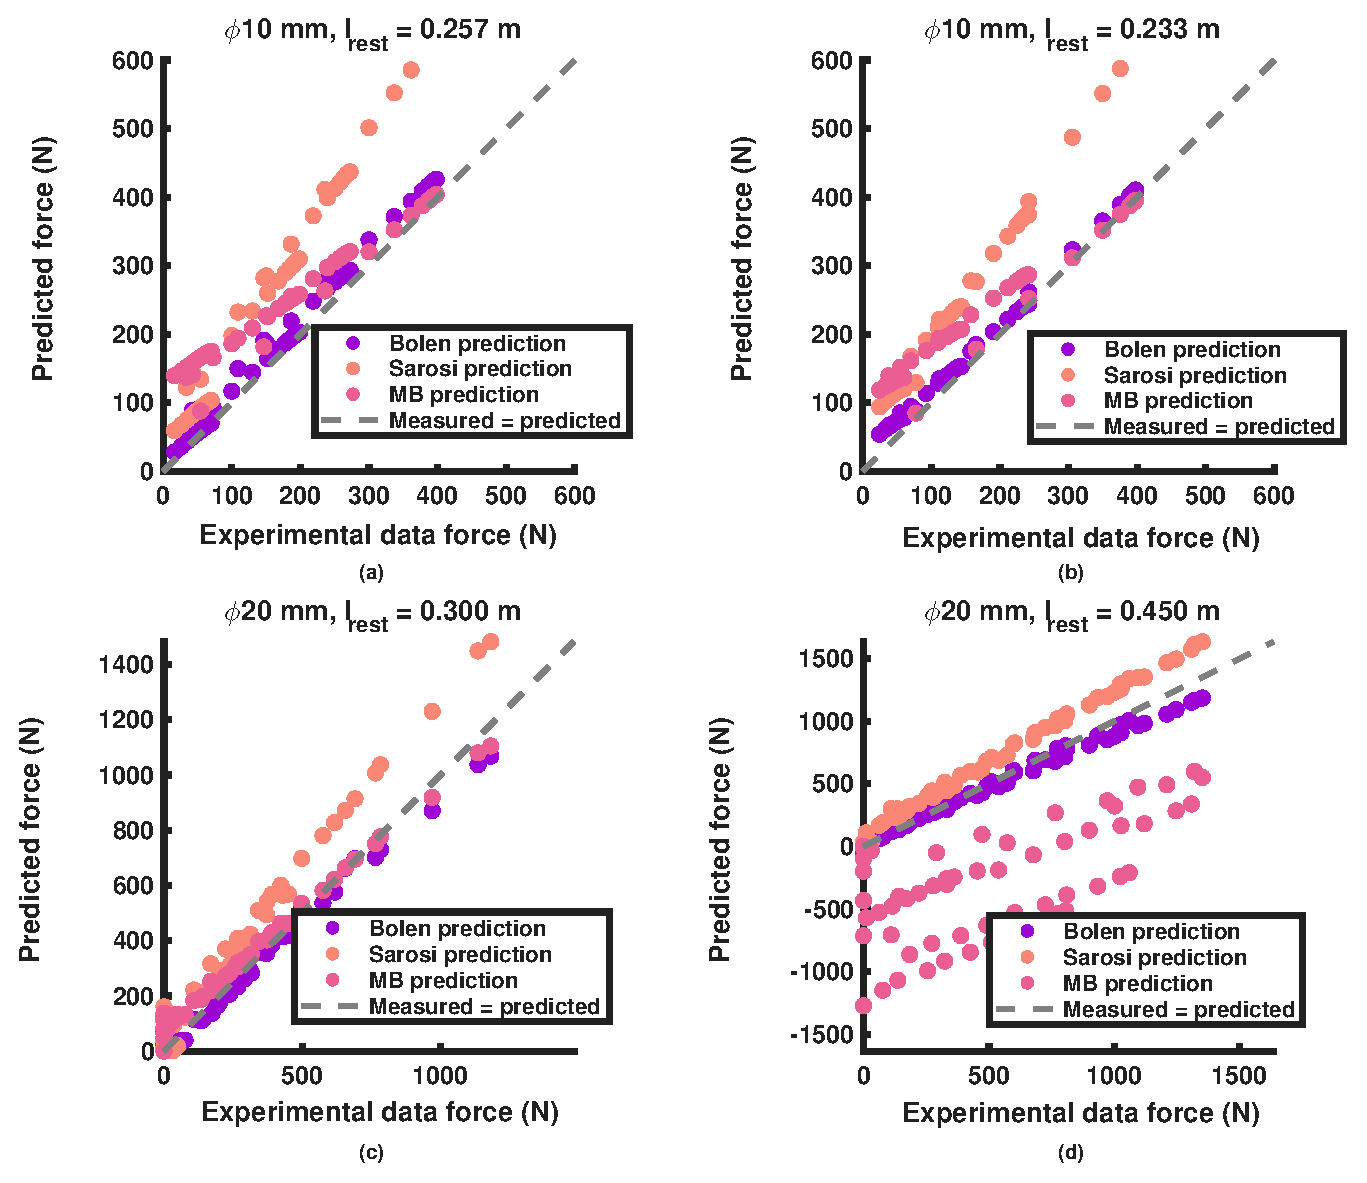
\includegraphics[width=.99\textwidth]{05_Comparison.eps}
%\end{center}
%\end{adjustwidth}
\caption{Comparison between measured and predicted BPA force at varying amounts of contraction and pressure. A $y=x$ perfect fit line is added for reference. The BPAs compared are: (\textbf{a}) $\diameter$\qty{10}{\mm}, $l_0=\qty{257}{\mm}$, (\textbf{b}) $\diameter$\qty{10}{\mm}, $l_0=\qty{233}{\mm}$, (\textbf{c}) $\diameter$\qty{20}{\mm}, $l_0=\qty{300}{\mm}$, and (\textbf{d}) $\diameter$\qty{20}{\mm}, $l_0=\qty{450}{\mm}$.}\label{fig:ModelCompare}
\end{figure}

The Martens and Boblan model was first evaluated at the same pressure–contraction points as in their experimental data \citep{martens_modeling_2017} (Tables A1 and  A2), indicating that it reproduces the general published force map shape but is sensitive to the assumed initial geometry. Examining their $\diameter$\qty{20}{\mm} BPA, for example, using the explicitly stated $l_0=\qty{300}{\mm}$ and initial diameter $D_{0}=\qty{20}{\mm}$ significantly under-predicted the results compared to using the implied $l_0=\qty{296}{\mm}$ (\citep{martens_modeling_2017} (Table A1)) and $D_{0}+H_{0}=\qty{21.8}{\mm}$, where $H_{0}=\qty{1.8}{\mm}$ is the material thickness. The diameter adjustment can be inferred \mbox{from \citep{chou_measurement_1996}.} This adjusted diameter was also included for the $\diameter$\qty{10}{\mm} BPA to give a better fit. As can be seen in Figure~\ref{fig:ModelCompare} and Table~\ref{tab:model_compare}, the highest accuracy is observed when $\diameter$\qty{20}{\mm} and $l_0=\qty{300}{\mm}$, which is at or very near their experimental measurements. For the $\diameter$\qty{10}{\mm} BPAs the accuracy decreases even though their experimentally measured $l_0=\qty{250}{\mm}$ is close to our $l_0=\qty{257}{\mm}$ and $l_0=\qty{233}{\mm}$. The largest error occurs at $\diameter$\qty{20}{\mm} and $l_0=\qty{450}{\mm}$ and the model starts to predict negative force. We have calculated that the $F_{PE}\cdot\frac{dD}{DL}$ term becomes very large compared to the others \citep{martens_modeling_2017} (p.~5). This suggests that the model is sensitive to geometric parameter selection and interpretation, particularly with respect to initial length and diameter definitions.

In comparison, the present normalized model demonstrates improved consistency across actuator lengths by incorporating experimentally derived scaling through $F_{620}$ and $\epsilon_{620}$. This normalization reduces sensitivity to geometric variation and enables a unified representation of actuator behavior, while maintaining predictive accuracy over the tested range of pressures and contractions.

\subsection{Implications for Real-Time Control and Simulation}

Although pneumatic muscle actuators exhibit hysteresis, thermodynamic effects, and other dynamic behavior, accurate and high-performance controller designs can still be achieved using a static force map approach when the underlying static force model is accurate. Martens and Boblan explicitly note that BPA dynamics are often dominated by the air dynamics inside the actuator and the mass flow behavior of the valve, such that precise modeling of the static force characteristic remains crucial for torque control \mbox{accuracy \citep{martens_modeling_2017}.} This view is consistent with more recent BPA control work, including a sensor-less torque control interface for BPA-driven joints \citep{martens_framework_2018}, stable force/position/stiffness control of antagonistic pneumatic-muscle joints \citep{ugurlu2019stable, hunt_development_2017}, and sensor-less angle stiffness control of antagonistic BPA systems \citep{shinSensorlessAngleStiffness2022}. 

In this context, the present model is well suited for real-time use because it reduces the static isometric force prediction to a low-order normalized surface, $F^*(\epsilon^*,P^*)$, scaled by the resting-length-dependent term $F_{620}(l_0)$. This structure is computationally inexpensive to evaluate online and is also suitable for lookup-table implementation. While the present work does not model the full actuator--valve dynamics, it provides the static force relationship needed as a feedforward or inner-model component in real-time torque control, simulation, and preliminary design workflows. It is anticipated that improved real-time control for high-speed and high-precision systems will benefit more from improved modeling of airflow dynamics than from modeling actuator hysteresis, damping, and other dynamic behavior. Characterizing the actuators under dynamic operating conditions, such as isokinetic (constant-velocity), isobaric, and isotonic (constant-load) contractions, is a natural next step beyond the isometric characterization reported here, for which the pressure--force dynamics model of \citet{elzein_pressure_2025} provides the modeling foundation.


\subsection{Biomimetic Artificial Muscle Analogy}\label{sec:disc_bio}

BPA artificial muscles are often said to be analogous to biological muscles because they have force--length curves and can produce force only in tension. This analogy is worth closer inspection. For example, the passive force–length curve has been described as an exponential function arising from connective tissue elements, while the active force–length relationship is typically modeled as a bell-shaped curve reflecting actin–myosin overlap \citep{winters1990}. These formulations emphasize that muscle force generation is governed by nonlinear geometric and material interactions rather than simple linear elasticity.
McKibben-type pneumatic artificial muscles (of which Festo is an example) exhibit analogous nonlinear behavior, though arising from fundamentally different physical mechanisms. As shown by Chou and Hannaford, the force–length relationship of McKibben actuators is derived from geometric constraints imposed by the braided shell, leading to a nonlinear dependence of force on actuator length through the braid angle \cite{chou_measurement_1996}. In their formulation, actuator force is proportional to pressure and a nonlinear geometric term $(3\cos^2\theta - 1)$, which governs both the maximum contraction limit and the curvature of the force–length relationship. The work presented here demonstrates that this nonlinear curve can be well approximated by an exponential as well.

However, the behavior of these artificial muscles differs distinctly from that of biological muscles.
For example, the optimal fiber length of a biological muscle, $l_{OFL}$, is not equivalent to $l_0$ in an artificial muscle. Artificial muscles produce their maximum active force at their resting length, which is also their maximum length. In contrast, the maximum active force that a biological muscle can produce is somewhere in the middle of the total contractile length of the muscle. 

Furthermore, biological muscles can adapt the optimal operating length through structural remodeling (e.g., sarcomere addition or tendon compliance) while BPAs have a fixed geometric configuration. This allows biological systems to self-optimize for the particular tasks the animal is subjected to. In order to re-optimize a robot for new tasks, new actuators would have to be swapped into the system. This distinction highlights a key limitation of BPAs in biomimetic applications, while also reinforcing the importance of accurate nonlinear modeling for control and design.

The analogy also suggests two design observations. First, the force--length penalty is shared by both families: force falls as the actuator operates away from its optimum, so a limb design must route each actuator such that its highest-force operating range coincides with the joint angles where torque is needed most, because the force lost at the extremes of the range of motion cannot be recovered by pressure alone. Second, the two families gain moment arm in different ways. Skeletal muscle attaches to the skeleton itself, through tendons or directly over broad areas of bone, so the moment arms of large animals follow from skeletal geometry. The robot's BPAs instead act through brackets that protrude from the limb segments; that hardware is mechanically exposed, and its series compliance is one of the loss mechanisms quantified in Chapter~\ref{ch:torque}.

The analogy finally raises a question that this dissertation can pose but not settle. Every muscle-like actuator loses force as it operates away from its optimal length, and a soft actuator working against soft structure has no rigid skeleton from which to gain a moment arm. Given those two facts, it may be no accident that nearly all large land animals are built on rigid skeletons and that large soft-bodied land animals are essentially absent. Whether the force--length penalty contributes to that absence, or whether it reflects other constraints such as support and protection, is a question for comparative biomechanics rather than for a single actuator study. For the designer, the lesson holds regardless of the answer: some moment arm must come from somewhere, and on this robot it comes from protruding brackets whose behavior must be modeled rather than ignored.

